\chapter{Masses des fermions : chiralité, couplages de Yukawa et neutrinos de Majorana}

\lectureoverview{Nous reprenons d’abord le mécanisme de Higgs des bosons de jauge dans une théorie jouet \(U(1)\), puis nous posons la question analogue pour les fermions. Une masse de Dirac mélange des champs de chiralités gauche et droite, mais l’interaction faible leur attribue des charges différentes et interdit donc un terme de masse nu. Un couplage de Yukawa au champ de Higgs respecte la symétrie ; après que le champ de Higgs a acquis une valeur dans le vide, cette même interaction devient une masse fermionique et un couplage mesurable entre le Higgs et le fermion--. La dernière partie prolonge ce raisonnement à la masse des neutrinos, aux particules lourdes éventuellement non protégées, à la cinématique des rayons cosmiques, à l’inertie relativiste et à la gravité.}

Le récapitulatif initial ne vise pas simplement à répéter le cours précédent. Nous avons besoin d’une de ses idées, formulée de façon à pouvoir être transposée aux fermions : une masse correspond à une énergie non nulle pour une excitation de quantité de mouvement nulle. Pour un champ, une quantité de mouvement nulle signifie une longueur d’onde infinie, autrement dit un déplacement identique en tout point. Une théorie où n’apparaissent que des dérivées ne peut pas détecter un déplacement uniforme. Un terme sans dérivées, lui, le peut.

\section{L’histoire des bosons de jauge en un seul passage}

\subsection{Énergie cinétique et vecteur sans masse}

Le champ de jauge du modèle est \(A_\mu\), de tenseur de champ \begin{equation}
  F_{\mu\nu}
  =\partial_\mu A_\nu-\partial_\nu A_\mu .
  \label{eq:l09-field-strength}
\end{equation}Le tableau note schématiquement le terme cinétique de jauge \(F^2\). Avec une normalisation usuelle, il s’écrit \begin{equation}
  \mathcal L_{\mathrm{gauge}}
  =-\frac14 F_{\mu\nu}F^{\mu\nu}.
  \label{eq:l09-gauge-kinetic}
\end{equation}

\begin{figure}[htbp]\centering
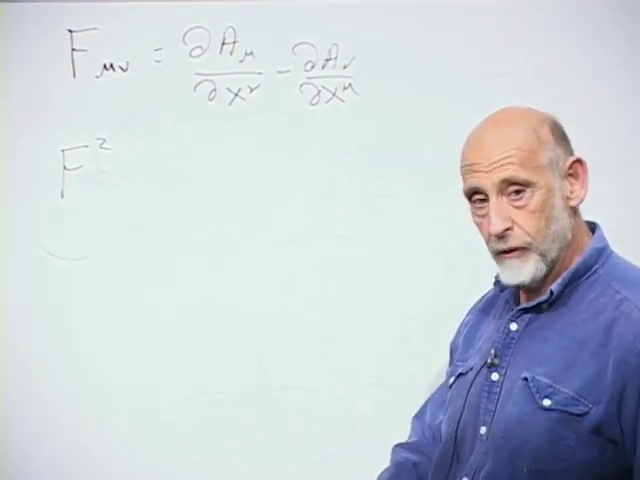
\includegraphics[width=0.72\textwidth]{lecture_09_figure_02.png}\caption{La définition du tenseur de champ et la notation abrégée \(F^2\) utilisée au tableau pour l’énergie cinétique du champ de jauge.}\lectureframe{00:02:39}\label{fig:l09-field-strength-board}\end{figure}

Dans \eqref{eq:l09-gauge-kinetic}, chaque occurrence de \(A_\mu\) est dérivée. Par conséquent, \begin{equation}
  A_\mu(x)\longmapsto A_\mu(x)+c_\mu,
  \qquad \partial_\nu c_\mu=0,
\end{equation} ne modifie pas \(F_{\mu\nu}\). Un potentiel vecteur homogène n’a donc pas d’énergie de champ associée. Dans le langage du cours, le mode de quantité de mouvement nulle n’a pas de gap et le boson de jauge est sans masse.

Ce champ \(U(1)\) est un modèle volontairement simplifié. Les particules visées sont \(W^\pm\) et \(Z\), et non le photon électromagnétique. La symétrie électromagnétique non brisée laisse le photon sans masse ; la symétrie électrofaible brisée donne une masse aux bosons de jauge faibles.

\subsection{Geler le rayon du champ de Higgs}

Introduisons un scalaire complexe chargé et écrivons-le sous forme polaire : \begin{equation}
  \phi(x)=\rho(x)e^{i\alpha(x)}.
\end{equation}Son potentiel en chapeau mexicain est minimal sur un cercle de rayon non nul. Appelons ce rayon \(f\) ; la direction radiale est relativement rigide. Pour commencer, nous la gelons et ne conservons que la phase : \begin{equation}
  \phi(x)\simeq f e^{i\alpha(x)}.
  \label{eq:l09-frozen-higgs}
\end{equation}

\begin{figure}[htbp]\centering
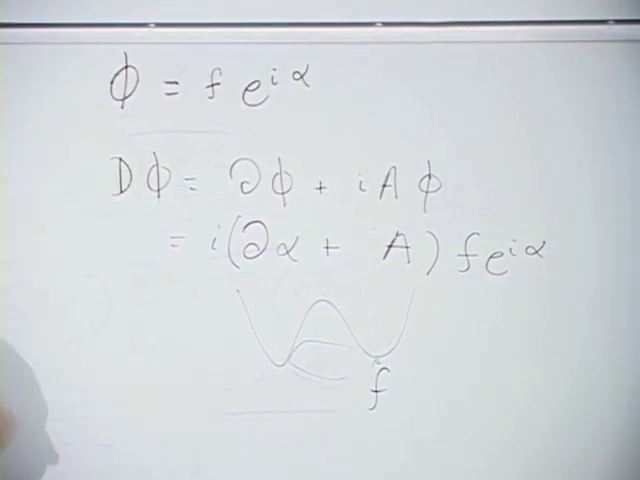
\includegraphics[width=0.72\textwidth]{lecture_09_figure_03.png}\caption{Le rayon gelé du champ de Higgs, sa dérivée covariante et le petit schéma du potentiel brisé utilisés dans le récapitulatif.}\lectureframe{00:06:42}\label{fig:l09-frozen-board}\end{figure}

Adoptons la convention \begin{equation}
\begin{aligned}
  D_\mu&=\partial_\mu+igA_\mu,
  \\
  \phi&\longmapsto e^{i\theta}\phi,
  \\
  A_\mu&\longmapsto A_\mu-\frac1g\partial_\mu\theta .
\end{aligned}
  \label{eq:l09-gauge-convention}
\end{equation}Le cours omet \(g\) ; l’écrire explicitement rend les dimensions et la masse qui apparaîtra ensuite plus transparentes. En agissant sur le champ gelé, on obtient \begin{align}
  D_\mu\phi
  &=(\partial_\mu+igA_\mu)f e^{i\alpha}
  \notag\\
  &=i\bigl(\partial_\mu\alpha+gA_\mu\bigr)
    f e^{i\alpha}.
  \label{eq:l09-covariant-frozen}
\end{align}La multiplication par le complexe conjugué élimine la phase et transforme aussi \(i\) fois \(-i\) en \(+1\) : \begin{equation}
  |D_\mu\phi|^2
  =f^2
   \bigl(\partial_\mu\alpha+gA_\mu\bigr)
   \bigl(\partial^\mu\alpha+gA^\mu\bigr).
  \label{eq:l09-frozen-square}
\end{equation}

\begin{classroomqa}\audiencequestion{Le carré de la dérivée covariante doit-il comporter un signe moins, puisque la dérivée a produit un facteur \(i\) ?\lecturetimestamp{00:07:39}}\lecturerresponse{Non. Le terme cinétique est le produit par le complexe conjugué. Un facteur contribue \(i\), l’autre \(-i\), et \(i(-i)=1\). On peut inverser de façon cohérente la convention de signe de \(D_\mu\), mais le carré du module est positif dans l’expression correspondante de l’énergie.}\end{classroomqa}

La combinaison dans \eqref{eq:l09-frozen-square} est elle-même un champ de jauge décalé. Choisissons \(\theta=-\alpha\), de sorte que la phase du scalaire disparaisse, et définissons \begin{equation}
  A'_\mu=A_\mu+\frac1g\partial_\mu\alpha .
  \label{eq:l09-unitary-gauge-field}
\end{equation}On a alors \begin{equation}
  |D_\mu\phi|^2=g^2f^2 A'_\mu A'^\mu .
  \label{eq:l09-vector-mass-term}
\end{equation}Ce nouveau terme ne contient aucune dérivée de \(A'_\mu\). Un champ homogène porte désormais de l’énergie : le mode vectoriel de quantité de mouvement nulle est donc doté d’un gap.

\begin{figure}[htbp]\centering
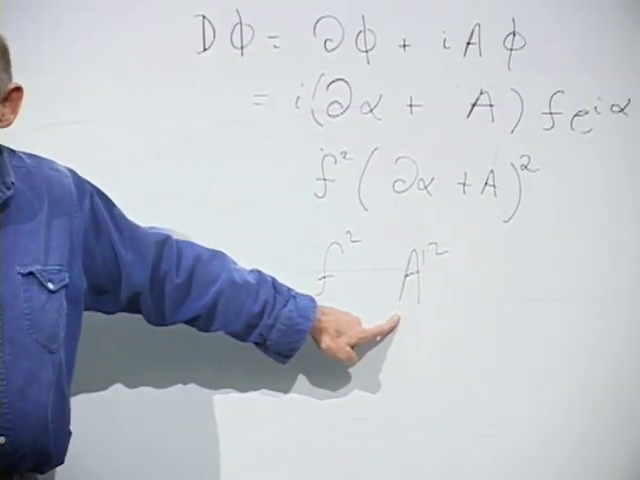
\includegraphics[width=0.72\textwidth]{lecture_09_figure_04.png}\caption{Le tableau isole le terme \(f^2A^2\) qui signale une masse pour le boson de jauge après absorption de la phase.}\lectureframe{00:10:31}\label{fig:l09-vector-mass-board}\end{figure}

Avec une normalisation canonique du scalaire, on écrit \(\phi=(f+h)e^{i\pi/f}/\sqrt2\). En comparant le terme vectoriel obtenu à \(\tfrac12m_A^2A_\mu A^\mu\), on trouve \begin{equation}
  m_A=gf
  \label{eq:l09-abelian-vector-mass}
\end{equation}dans ce modèle abélien. Le cours omet les facteurs de normalisation et résume le résultat en disant que la masse du vecteur est fixée par \(f\).

La phase ne disparaît pas sans contrepartie. Avant la mise sous jauge, elle correspondait à un boson de Goldstone sans masse. Après la mise sous jauge, elle fournit la polarisation longitudinale nécessaire à une particule vectorielle massive. La fluctuation radiale, que nous avions temporairement gelée, subsiste comme excitation physique du Higgs.

\subsection{Pourquoi un terme sans dérivées signifie une masse}

\begin{classroomqa}\audiencequestion{Pourquoi un terme \(A'^2\) compte-t-il comme une masse plutôt que comme une simple interaction supplémentaire ?\lecturetimestamp{00:13:10}}\lecturerresponse{Une masse est une énergie au repos. Pour un champ, une particule au repos est le quantum d’un mode de quantité de mouvement nulle et de longueur d’onde infinie. Le terme dérivé ne confère aucune énergie à un déplacement homogène statique, alors que \(m_A^2A'^2\) le fait. Cette énergie non nulle à quantité de mouvement nulle constitue le gap d’énergie de masse au repos.}\end{classroomqa}

Le cours développe cette idée à l’aide de trois analogies mécaniques.

\begin{itemize}\item Dans un cristal, un déplacement lentement variable coûte de l’énergie élastique, car les atomes voisins ne sont pas déplacés de la même façon. Une translation rigide déplace tous les atomes ensemble et ne coûte aucune énergie interne. Le phonon acoustique est donc sans gap.
  \item Dans un aimant idéalement invariant par rotation, une orientation de spin qui varie dans l’espace coûte de l’énergie d’échange, mais faire tourner ensemble tous les spins n’en coûte pas. L’onde de spin correspondante, de grande longueur d’onde, est sans gap.
  \item Dans un plasma, le déplacement du fluide électronique par rapport au fond positif crée une séparation de charges et un champ électrique de rappel, même pour un déplacement relatif homogène. Le plasmon qui en résulte possède une fréquence non nulle à nombre d’onde nul.
\end{itemize}

Le champ de jauge ayant acquis une masse se comporte comme dans le troisième exemple : le milieu brisé s’oppose à ce qui serait autrement un déplacement homogène sans coût énergétique.

\begin{classroomqa}\audiencequestion{Avant l’introduction du champ de jauge, la phase \(\alpha\) ne vibrait-elle pas déjà ?\lecturetimestamp{00:18:24}}\lecturerresponse{Si. Son énergie était proportionnelle à \(f^2(\partial_\mu\alpha)^2\). Une phase qui varie d’un point à l’autre possède une énergie de gradient et peut se propager, mais une variation uniforme de la phase ne coûte rien. C’est précisément le mode de Goldstone sans masse.}\end{classroomqa}

\begin{classroomqa}\audiencequestion{La dérivée comprend une dérivée temporelle. Le fait de mettre réellement tout le réseau en mouvement ou de modifier tout le champ n’entraîne-t-il pas une énergie cinétique ?\lecturetimestamp{00:22:18}}\lecturerresponse{Si. La comparaison porte sur des configurations statiques, ou préparées aussi lentement que l’on veut. Un réseau qui se déplace à vitesse non nulle possède une énergie cinétique. Le critère de masse consiste à demander si la configuration conserve une énergie lorsqu’elle est au repos et uniforme dans l’espace.}\end{classroomqa}

\section{L’indice expérimental : les interactions faibles distinguent la gauche de la droite}

Le cours passe maintenant à l’électron, au muon et aux quarks. Leur masse provient elle aussi du champ de Higgs, mais le mécanisme prend une autre forme, car une masse fermionique n’est pas un terme quadratique vectoriel. C’est un couplage entre deux champs de chiralités différentes.

\subsection{La violation de la parité dans la désintégration bêta}

Partons du fait expérimental que l’interaction faible viole la parité. L’électrodynamique quantique et la chromodynamique quantique traitent de la même façon un processus et son image miroir. Ce n’est pas le cas de l’interaction faible. Dans la désintégration bêta du neutron, \begin{equation}
  n\longrightarrow p+e^-+\bar\nu_e,
  \label{eq:l09-beta-decay}
\end{equation}les électrons de haute énergie sélectionnés par l’interaction à courant chargé ont une hélicité gauche : leur spin est dirigé à l’opposé de leur quantité de mouvement. Les antineutrinos correspondants ont l’hélicité opposée.

Pour une particule ultrarelativiste, définissons l’hélicité par \begin{equation}
  h=\frac{\bm S\cdot\bm p}{|\bm S|\,|\bm p|}.
\end{equation}Un spin parallèle à la quantité de mouvement correspond à \(h=+1\) ; un spin antiparallèle, à \(h=-1\). L’interaction faible se couple à un champ électronique de chiralité gauche et à un champ de neutrino de chiralité gauche, mais pas de la même façon à un champ électronique de chiralité droite.\editorialnote{Au début, le cours parle de gauche et de droite au sens de l’hélicité, car cette image est intuitive à haute énergie. En réalité, les charges de jauge agissent sur la chiralité, c’est-à-dire l’étiquette de représentation de Lorentz sélectionnée par \(P_L=(1-\gamma^5)/2\) et \(P_R=(1+\gamma^5)/2\). Pour une particule sans masse, chiralité et hélicité coïncident ; pour une particule massive, elles ne coïncident pas.}

Pour mettre en évidence l’obstacle sans introduire tout l’appareil de \(SU(2)_L\times U(1)_Y\), imaginons un monde fictif \(U(1)\) où seul \(\psi_L\) porte la charge pertinente : \begin{equation}
  \psi_L\longmapsto e^{i\theta}\psi_L,
  \qquad
  \psi_R\longmapsto\psi_R .
  \label{eq:l09-chiral-toy-charge}
\end{equation}Ce n’est pas l’électromagnétisme : dans la réalité, les électrons de chiralité gauche et droite portent la même charge électrique. Il s’agit d’une caricature de l’interaction faible, où les deux chiralités appartiennent à des représentations électrofaibles différentes.

\begin{classroomqa}\audiencequestion{La même asymétrie gauche--droite s’applique-t-elle aux quarks ?\lecturetimestamp{00:31:50}}\lecturerresponse{Oui, avec les multiplets faibles et les hypercharges appropriés. Les quarks de type haut et de type bas de chiralité gauche forment des doublets faibles, tandis que les champs de chiralité droite sont des singulets faibles. Leurs couplages au Higgs rencontrent donc le même problème structurel que celui de l’électron.}\end{classroomqa}

\section{Une masse de Dirac mélange les chiralités gauche--droite}

\subsection{De l’équation à quatre composantes aux deux équations de Weyl}

Une fonction d’onde de Dirac possède quatre composantes. De façon schématique, deux décrivent le spin et deux distinguent les solutions d’énergie positive et négative, ces dernières étant réinterprétées comme des degrés de liberté d’antiparticule. Sous forme hamiltonienne, \begin{equation}
  i\frac{\partial\Psi}{\partial t}
  =\left(-i\bm\alpha\cdot\bm\nabla+m\beta\right)\Psi .
  \label{eq:l09-dirac-hamiltonian}
\end{equation}Les matrices \(\alpha_i\) et \(\beta\) encodent la relation relativiste entre l’énergie, la quantité de mouvement et la masse.

\begin{figure}[htbp]\centering
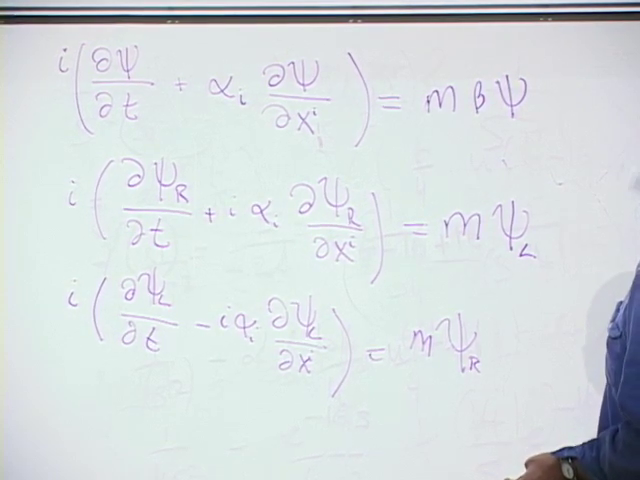
\includegraphics[width=0.74\textwidth]{lecture_09_figure_05.png}\caption{Le tableau écrit d’abord l’équation de Dirac, puis la décompose en équations couplées pour les champs de chiralités gauche et droite.}\lectureframe{00:40:30}\label{fig:l09-dirac-board}\end{figure}

La base chirale rend explicite le rôle de \(m\). Avec \(\sigma^\mu=(1,\bm\sigma)\) et \(\bar\sigma^\mu=(1,-\bm\sigma)\), on obtient \begin{align}
  i\bar\sigma^\mu\partial_\mu\psi_L&=m\psi_R,
  \label{eq:l09-weyl-left}\\
  i\sigma^\mu\partial_\mu\psi_R&=m\psi_L.
  \label{eq:l09-weyl-right}
\end{align}Pour \(m=0\), les équations sont indépendantes : un champ de chiralité gauche et un champ de chiralité droite peuvent se propager sans interagir. Pour \(m\neq0\), chacun devient la source de l’autre. C’est en ce sens précis qu’une masse de Dirac mélange les chiralités gauche et droite.

Susskind décrit cela en disant que le fermion oscille entre la gauche et la droite. Cette image rend compte du couplage, mais il ne faut pas la prendre au pied de la lettre et imaginer une particule ponctuelle classique qui basculerait d’un côté à l’autre. L’énoncé précis est l’équation de champ couplée \eqref{eq:l09-weyl-left}--\eqref{eq:l09-weyl-right}.

\begin{classroomqa}\audiencequestion{Les facteurs \(i\) et les signes des deux équations au tableau sont-ils cohérents ?\lecturetimestamp{00:41:10}}\lecturerresponse{Pas terme à terme au tableau : lors de la dérivation rapide, un facteur \(i\) a été sorti de façon incohérente. Le résultat fiable est la structure du couplage. Les équations \eqref{eq:l09-weyl-left} et \eqref{eq:l09-weyl-right} correspondent à une convention cohérente usuelle.}\end{classroomqa}

\subsection{Pourquoi la symétrie faible interdit une masse nue}

Le terme de masse de Dirac correspondant dans le lagrangien est \begin{equation}
  \mathcal L_m
  =-m\bar\psi\psi
  =-m\left(\bar\psi_L\psi_R+\bar\psi_R\psi_L\right).
  \label{eq:l09-bare-dirac-mass}
\end{equation}Sous la transformation jouet \eqref{eq:l09-chiral-toy-charge}, on a \begin{equation}
  \bar\psi_L\psi_R\longmapsto
  e^{-i\theta}\bar\psi_L\psi_R,
  \qquad
  \bar\psi_R\psi_L\longmapsto
  e^{i\theta}\bar\psi_R\psi_L.
\end{equation}Aucun des deux termes n’est invariant. Le coefficient du mélange direct gauche--droite \(m\) est donc interdit avant la brisure de symétrie.

L’électromagnétisme seul ne poserait pas ce problème, puisque \(\psi_L\) et \(\psi_R\) portent la même charge électrique. L’obstacle vient de leurs nombres quantiques faibles différents.

\subsection{Questions sur l’hélicité qui mettent en évidence les subtilités de la chiralité}

Le cours met maintenant à l’épreuve l’image intuitive des chiralités sous différents angles. Ces questions ne sont pas secondaires : elles montrent précisément dans quels cas l’hélicité est utile et dans quels cas il faut parler de chiralité.

\begin{classroomqa}\audiencequestion{À quoi ressemblerait le monde si l’interaction faible produisait les deux hélicités de l’électron en quantités égales ?\lecturetimestamp{00:42:12}}\lecturerresponse{L’asymétrie de parité immédiate disparaîtrait dans ce processus. Mais la véritable théorie électrofaible est chirale : seuls les doublets de chiralité gauche portent l’interaction faible à courant chargé. Le cours remet à plus tard une explication plus complète de la raison pour laquelle la nature a adopté cette structure.}\end{classroomqa}

\begin{classroomqa}\audiencequestion{Supposons que le spin d’un électron soit préparé verticalement, puis que l’électron soit accéléré horizontalement. Est-il de chiralité gauche ou droite ?\lecturetimestamp{00:42:44}}\lecturerresponse{Un état de spin transverse à la quantité de mouvement est une superposition des deux hélicités. L’hélicité est bien définie uniquement lorsque le spin est parallèle ou antiparallèle à la quantité de mouvement. Les projecteurs chiraux faibles restent néanmoins bien définis pour le champ.}\end{classroomqa}

Une particule massive peut être ralentie jusqu’à l’arrêt, puis accélérée dans la direction opposée sans que son spin s’inverse. Son hélicité change alors de signe. Une particule sans masse ne peut être rattrapée ni arrêtée par une transformation de Lorentz ; son hélicité est donc invariante sous les boosts propres. Cela motive l’affirmation du cours selon laquelle une espèce qui ne possède qu’une seule hélicité physique doit être sans masse. L’énoncé plus précis, en théorie des champs, est qu’une masse de Dirac invariante de Lorentz nécessite les deux chiralités.

\begin{classroomqa}\audiencequestion{Un photon polarisé circulairement peut se réfléchir sur un miroir et inverser sa direction sans jamais s’arrêter. Est-ce en contradiction avec l’argument sur l’hélicité ?\lecturetimestamp{00:45:28}}\lecturerresponse{Non. Le miroir est un système extérieur qui peut échanger du moment angulaire et inverser la direction de propagation. Une réflexion n’est pas un boost de Lorentz qui rattrape le photon. L’existence d’un canal dépend aussi des états de polarisation permis et des conditions aux limites du matériau.}\end{classroomqa}

\begin{classroomqa}\audiencequestion{Un faisceau ordinaire d’électrons contient-il une seule chiralité ou les deux ?\lecturetimestamp{00:46:10}}\lecturerresponse{En général, les deux. Un état d’électron massif contient les deux composantes chirales, et un faisceau non polarisé contient les deux hélicités. Des sources spécialisées peuvent produire un faisceau polarisé présentant une forte asymétrie d’hélicité.}\end{classroomqa}

\begin{classroomqa}\audiencequestion{Peut-on focaliser un faisceau indépendamment de son spin, ou les champs magnétiques séparent-ils les deux polarisations ?\lecturetimestamp{00:46:29}}\lecturerresponse{La focalisation ordinaire en position peut être largement indépendante du spin, mais les moments magnétiques se couplent aux gradients du champ magnétique. Des sources sélectives en spin, des gradients de type Stern--Gerlach et la dynamique du spin dans les accélérateurs peuvent donc préparer ou séparer les polarisations.}\end{classroomqa}

\begin{classroomqa}\audiencequestion{La différence entre gauche et droite dans l’interaction faible est-elle simplement un accident ?\lecturetimestamp{00:48:13}}\lecturerresponse{Dans le cadre de ce cours, c’est un fait expérimental intégré au Modèle standard. Cette différence est trop systématique pour sembler due au hasard, mais le Modèle standard lui-même ne déduit pas la structure complète des charges chirales à partir d’un principe plus profond.}\end{classroomqa}

\section{La construction de Yukawa}

\subsection{Attribuer au Higgs la charge manquante}

La symétrie interdit une masse numérique, mais autorise une interaction avec un champ qui fournit la phase de transformation manquante. Introduisons un scalaire complexe tel que \begin{equation}
  \phi\longmapsto e^{i\theta}\phi,
  \qquad
  \phi^\dagger\longmapsto e^{-i\theta}\phi^\dagger.
  \label{eq:l09-scalar-charge}
\end{equation}Alors \begin{equation}
  \mathcal L_Y
  =-y\,\bar\psi_L\phi\psi_R
   -y^*\,\bar\psi_R\phi^\dagger\psi_L
  \label{eq:l09-yukawa-lagrangian}
\end{equation}est invariant de jauge. Dans le premier terme, \(\bar\psi_L\) contribue \(e^{-i\theta}\) et \(\phi\) contribue \(e^{i\theta}\) ; les phases se compensent. Le second terme est son conjugué hermitien.

De façon équivalente, les équations chirales acquièrent un mélange dépendant du champ : \begin{align}
  i\bar\sigma^\mu D_\mu\psi_L
    &=y\phi\psi_R,
  \label{eq:l09-yukawa-eom-left}\\
  i\sigma^\mu\partial_\mu\psi_R
    &=y^*\phi^\dagger\psi_L.
  \label{eq:l09-yukawa-eom-right}
\end{align}

\begin{figure}[htbp]\centering
\includegraphics[width=0.76\textwidth]{lecture_09_figure_06.png}\caption{Le terme de masse nu dans les membres de droite a été remplacé par le champ scalaire chargé. Les signes exacts du tableau sont schématiques ; la structure invariante est donnée par \eqref{eq:l09-yukawa-lagrangian}.}\lectureframe{00:51:30}\label{fig:l09-yukawa-board}\end{figure}

Avant la brisure de symétrie, il s’agit d’une interaction, et non d’une masse. Un fermion de chiralité droite ne peut devenir un fermion de chiralité gauche qu’en émettant ou en absorbant le quantum scalaire nécessaire pour équilibrer la charge. Le coefficient \(y\) est un couplage de Yukawa, et non la charge de jauge \(g\).

\begin{classroomqa}\audiencequestion{Peut-on simplement ajouter \(\phi\) et \(\phi^\dagger\) aux membres de droite des deux équations ?\lecturetimestamp{00:51:55}}\lecturerresponse{Oui, précisément parce que leurs phases de transformation corrigent le désaccord. Le critère décisif n’est pas la forme visuelle de l’équation, mais l’invariance de jauge de l’interaction \(\bar\psi_L\phi\psi_R+\mathrm{h.c.}\).}\end{classroomqa}

\subsection{Le vide transforme l’interaction en masse}

Identifions maintenant \(\phi\) au champ de Higgs et laissons-le s’établir avec un module non nul dans le vide. Avec la normalisation simplifiée du cours, \begin{equation}
  \phi\simeq f,
\end{equation}et \eqref{eq:l09-yukawa-lagrangian} contient alors \begin{equation}
  \mathcal L_Y
  \supset
  -yf\,\bar\psi_L\psi_R
  -y^*f\,\bar\psi_R\psi_L .
\end{equation}Après une redéfinition de phase sans conséquence, si nécessaire, la masse du fermion est \begin{equation}
  m_f=yf.
  \label{eq:l09-lecture-fermion-mass}
\end{equation}C’est l’analogue fermionique du résultat vectoriel \(m_A=gf\). Le même vide de Higgs qui fournit une polarisation longitudinale aux bosons de jauge faibles apporte les nombres quantiques faibles manquants pour relier les fermions de chiralités gauche et droite.

Dans la convention du Modèle standard à normalisation canonique, \begin{equation}
  H(x)=\frac1{\sqrt2}
  \begin{pmatrix}
    0\\ v+h(x)
  \end{pmatrix},
  \qquad v\simeq246\ \mathrm{GeV},
  \label{eq:l09-sm-higgs-vacuum}
\end{equation}et par conséquent \begin{equation}
  m_f=\frac{y_fv}{\sqrt2}.
  \label{eq:l09-sm-fermion-mass}
\end{equation}La quantité \(f\) du cours et la quantité conventionnelle \(v/\sqrt2\) ne diffèrent que par ce choix de normalisation.

\begin{classroomqa}\audiencequestion{Si seul le produit \(yf\) constitue une masse fermionique, comment peut-on déterminer séparément le couplage \(y\) et l’échelle du vide \(f\) ?\lecturetimestamp{00:55:36}}\lecturerresponse{Les masses des bosons de jauge faibles déterminent l’échelle du vide une fois les couplages de jauge connus. La masse mesurée d’un fermion détermine ensuite son couplage de Yukawa. Dans la théorie complète, \(m_W=gv/2\), \(m_Z=v\sqrt{g^2+g'^2}/2\) et \(y_f=\sqrt2m_f/v\).}\end{classroomqa}

\begin{classroomqa}\audiencequestion{La masse du boson faible est-elle d’environ \(900\ \mathrm{GeV}\) ?\lecturetimestamp{00:57:43}}\lecturerresponse{Non ; le cours corrige aussitôt cette erreur et donne environ \(90\ \mathrm{GeV}\). Plus précisément, \(m_W\simeq80\ \mathrm{GeV}\) et \(m_Z\simeq91\ \mathrm{GeV}\), tandis que l’échelle sous-jacente du vide vaut \(v\simeq246\ \mathrm{GeV}\).}\end{classroomqa}

\subsection{Une échelle du vide, de nombreux couplages de Yukawa}

Chaque espèce de fermion chargé possède son propre couplage de Yukawa : \begin{equation}
  m_i=y_i f
  \qquad\text{(lecture normalization)}.
  \label{eq:l09-mass-family}
\end{equation}

\begin{figure}[htbp]\centering
\includegraphics[width=0.76\textwidth]{lecture_09_figure_08.png}\caption{Le tableau résume la dépendance en espèce par \(m_i=g_i f\) ; les \(g_i\) qui y figurent sont les couplages de Yukawa que nous notons \(y_i\) ici.}\lectureframe{01:16:30}\label{fig:l09-mass-family-board}\end{figure}

Pour l’électron, le cours estime \begin{equation}
  y_e\sim\frac{0.5\ \mathrm{MeV}}{10^2\ \mathrm{GeV}}
  \sim10^{-5}.
\end{equation}Avec la valeur canonique \(v=246\ \mathrm{GeV}\), on obtient une valeur plus précise : \(y_e\simeq2.9\times10^{-6}\). Le quark top se situe à l’autre extrémité : \begin{equation}
  y_t=\frac{\sqrt2m_t}{v}\simeq1.
\end{equation}Ainsi, le mécanisme de Higgs explique comment une masse invariante de jauge peut exister, mais il n’explique pas l’immense hiérarchie entre les \(y_i\). Les masses fermioniques observées ne font que traduire cette hiérarchie en valeurs mesurées.

\begin{classroomqa}\audiencequestion{Le couplage de Yukawa du quark top est-il vraiment de l’ordre de l’unité ?\lecturetimestamp{00:59:09}}\lecturerresponse{Oui. Sa masse est comparable à l’échelle électrofaible, de sorte que son couplage n’est pas un nombre perturbatif minuscule comme celui de l’électron. Avec la normalisation moderne, \(y_t\) est proche de l’unité.}\end{classroomqa}

\subsection{Rétablir la fluctuation physique du Higgs}

En gelant le scalaire à sa valeur dans le vide, nous avons masqué l’excitation radiale. Rétablissons-la de façon schématique : \begin{equation}
  \phi(x)\simeq f+h(x).
\end{equation}Le facteur de Yukawa devient \begin{equation}
  y\phi\simeq yf+yh=m_f+yh.
  \label{eq:l09-mass-plus-higgs}
\end{equation}

\begin{figure}[htbp]\centering
\includegraphics[width=0.76\textwidth]{lecture_09_figure_07.png}\caption{Le tableau rétablit la fluctuation du Higgs dans le terme de Yukawa : la partie constante produit la masse fermionique, et la partie fluctuante permet l’émission ou l’absorption d’un Higgs.}\lectureframe{01:01:15}\label{fig:l09-higgs-fluctuation-board}\end{figure}

Le premier terme de \eqref{eq:l09-mass-plus-higgs} est le terme de masse. Le second est un sommet où un boson de Higgs se couple au fermion. Dans la notation canonique du Modèle standard, \begin{equation}
  \mathcal L_Y
  \supset
  -m_f\bar\psi\psi
  -\frac{m_f}{v}h\bar\psi\psi.
  \label{eq:l09-higgs-fermion-vertex}
\end{equation}Le couplage est proportionnel à la masse du fermion. Sous réserve de la cinématique, des facteurs de couleur, de l’espace des phases et des canaux concurrents, le Higgs se couple donc plus fortement aux fermions lourds.

\begin{classroomqa}\audiencequestion{Les constantes de couplage sont-elles elles-mêmes des probabilités ?\lecturetimestamp{01:03:35}}\lecturerresponse{Elles interviennent dans les amplitudes quantiques. Un taux simple est souvent proportionnel au carré du module d’une amplitude et donc au carré d’un couplage, mais l’espace des phases, les sommes sur les spins, les interférences, les boucles et la multiplicité des sommets jouent aussi un rôle. Il ne faut pas identifier directement un couplage à une probabilité.}\end{classroomqa}

\begin{classroomqa}\audiencequestion{Cet argument suppose-t-il qu’il n’existe qu’un seul champ de Higgs ?\lecturetimestamp{01:03:59}}\lecturerresponse{Il décrit le Modèle standard minimal, qui possède un doublet de Higgs complexe. Trois de ses quatre composantes réelles sont absorbées par \(W^\pm\) et \(Z\), laissant un scalaire neutre physique. Des extensions peuvent comporter davantage de doublets ou d’autres multiplets scalaires. Les modèles supersymétriques nécessitent généralement deux doublets de Higgs et contiennent donc plusieurs états physiques du Higgs.}\end{classroomqa}

On peut maintenant confronter cette attente historique à l’expérience. \editorialnote{Ce cours a été enregistré avant la découverte du Higgs. ATLAS et CMS ont annoncé l’observation d’une particule de type Higgs en 2012, dont la masse est aujourd’hui mesurée à environ \(125\ \mathrm{GeV}\). Ses couplages observés sont globalement conformes au modèle du Modèle standard où les couplages sont proportionnels à la masse. L’affirmation selon laquelle il se désintègre préférentiellement en particules très lourdes doit toujours être assortie d’une réserve cinématique : une paire \(t\bar t\) est trop lourde pour un Higgs de \(125\ \mathrm{GeV}\).}

\section{Antiparticules, faisceaux et sens de la chiralité}

Avant d’aborder les neutrinos, le cours revient à plusieurs questions pratiques sur les antiparticules et les faisceaux d’accélérateur.

\begin{classroomqa}\audiencequestion{Quelle est la chiralité de l’antiparticule d’un électron de chiralité gauche ?\lecturetimestamp{01:06:05}}\lecturerresponse{Dans la limite ultrarelativiste, un champ électronique de chiralité gauche annihile des électrons d’hélicité gauche et crée des positrons d’hélicité droite. C’est un cas où il faut distinguer soigneusement particule et antiparticule, ainsi que chiralité et hélicité.}\end{classroomqa}

\begin{classroomqa}\audiencequestion{Un électron et un positron peuvent-ils entrer en collision pour produire un boson \(Z\) ?\lecturetimestamp{01:07:13}}\lecturerresponse{Oui, lorsque leur énergie dans le centre de masse correspond au canal autorisé. Les collisionneurs électron--positron ont étudié la résonance \(Z\) avec une grande précision. La charge et les autres nombres quantiques sont conservés dans le processus complet.}\end{classroomqa}

\begin{classroomqa}\audiencequestion{Les positrons sont-ils tous produits par un seul processus faible particulier ?\lecturetimestamp{01:07:37}}\lecturerresponse{Non. La création de paires est un mécanisme électromagnétique classique. Par exemple, un électron énergétique peut émettre un photon virtuel, lequel peut produire une paire \(e^-e^+\) dans le champ d’une autre particule. Le cours illustre ce processus par un diagramme de Feynman.}\end{classroomqa}

\begin{classroomqa}\audiencequestion{Un accélérateur linéaire peut-il sélectionner la vitesse ou l’énergie de ses électrons ?\lecturetimestamp{01:09:24}}\lecturerresponse{Oui. Les champs accélérateurs et leur synchronisation sélectionnent une gamme d’énergie. Une fois ultrarelativistes, les électrons ont déjà une vitesse extrêmement proche de \(c\) ; l’énergie supplémentaire fournie par l’accélérateur augmente donc surtout leur quantité de mouvement et leur énergie totale, sans accroître visiblement leur vitesse.}\end{classroomqa}

\begin{classroomqa}\audiencequestion{Un accélérateur peut-il préparer un faisceau d’une seule polarisation ?\lecturetimestamp{01:09:47}}\lecturerresponse{Oui, bien que ce soit techniquement difficile. On peut préparer à basse énergie des électrons polarisés en spin à l’aide d’une source dépendant du spin, puis les accélérer en contrôlant la précession du spin. Les collisionneurs modernes quantifient la polarisation obtenue au lieu de la considérer comme parfaitement pure.}\end{classroomqa}

\section{Masse des neutrinos et possibilité de Majorana}

\subsection{Pourquoi la masse des neutrinos a imposé une extension}

Le Modèle standard minimal d’origine ne comprenait que des champs de neutrinos de chiralité gauche et prédisait donc des neutrinos sans masse. Les oscillations des neutrinos montrent qu’au moins deux de leurs valeurs propres de masse diffèrent et que leur masse est non nulle, bien qu’infime par rapport à celle des fermions chargés.

\begin{classroomqa}\audiencequestion{Quelle est l’ordre de grandeur des masses des neutrinos, et où se trouve leur composante droite ?\lecturetimestamp{01:10:38}}\lecturerresponse{Les oscillations déterminent les différences des carrés des masses, et non les masses absolues. Les écarts pertinents correspondent à des échelles d’environ \(0.009\ \mathrm{eV}\) et \(0.05\ \mathrm{eV}\). Une description de Dirac ajoute des neutrinos de chiralité droite stériles ; une description de Majorana relie plutôt la chiralité manquante à des champs de neutrinos conjugués de charge.}\end{classroomqa}

Pour un neutrino de Dirac, on ajoute un nouveau champ \(\nu_R\) et on reprend la construction de Yukawa : \begin{equation}
  \mathcal L_{\nu,\mathrm{Dirac}}
  =-y_\nu\bar L\,\widetilde H\,\nu_R+\mathrm{h.c.},
  \qquad
  m_\nu=\frac{y_\nu v}{\sqrt2}.
  \label{eq:l09-dirac-neutrino}
\end{equation}Le \(y_\nu\) nécessaire est extraordinairement petit.

Il existe une autre possibilité logique, puisque le neutrino ne porte aucune charge électrique. Un neutrino de chiralité gauche peut se coupler à son propre conjugué de charge, qui a la chiralité opposée :
\begin{equation}
  \nu_L\longleftrightarrow(\nu_L)^c_R .
  \label{eq:l09-majorana-mixing}
\end{equation}
Un état propre de masse construit de cette manière est un fermion de Majorana : c’est sa propre antiparticule, à des conventions de phase près. Le mélange électron--positron analogue est interdit, car il violerait la conservation exacte de la charge électrique.

\begin{classroomqa}
\audiencequestion{Pourquoi le mélange particule--antiparticule est-il permis pour un neutrino, mais pas pour un électron ?\lecturetimestamp{01:13:43}}
\lecturerresponse{L’électron et le positron ont des charges électriques opposées ; un terme de masse qui les mélangerait en un même état à une particule violerait donc la symétrie électromagnétique non brisée. Le neutrino est électriquement neutre. Si aucun nombre leptonique conservé exactement ne le distingue de son antiparticule, une masse de Majorana est permise.}
\end{classroomqa}

Ce nom rend hommage à Ettore Majorana, jeune physicien italien qui a formulé ce type de représentation réelle des fermions et a disparu en 1938. Le cours s’arrête sur ce mystère historique : son sort n’a jamais été établi.
\editorialnote{Avant la brisure électrofaible, le neutrino actif du Modèle standard ne peut pas avoir de terme de masse de Majorana nu invariant de jauge et renormalisable. À basse énergie, une telle masse peut provenir de l’opérateur de Weinberg de dimension cinq
\((LH)(LH)/\Lambda\), ou d’un mécanisme de bascule faisant intervenir des neutrinos stériles lourds. La question de savoir si les neutrinos sont des particules de Dirac ou de Majorana n’est toujours pas tranchée expérimentalement.}

\section{Pourquoi le spectre familier se regroupe près de l’échelle électrofaible}

\subsection{L’échelle commune et ses importantes réserves}

\begin{classroomqa}
\audiencequestion{Pourquoi s’attendait-on à ce que la masse du Higgs soit accessible à l’échelle faible ?\lecturetimestamp{01:14:48}}
\lecturerresponse{La courbure du potentiel du Higgs détermine la masse radiale du Higgs, tandis que la même échelle du vide \(f\) détermine les masses des bosons \(W\) et \(Z\). En l’absence d’un couplage d’auto-interaction scalaire extrême, on s’attendait donc à ce que la masse du Higgs soit du même ordre général que l’échelle faible. La valeur observée, \(125\ \mathrm{GeV}\), se situe bien dans cette gamme.}
\end{classroomqa}

Le cours résume de façon frappante que les masses élémentaires du Modèle standard minimal remontent à un seul vide brisé :
\begin{align}
  m_W&=\frac12gv,\\
  m_Z&=\frac12\sqrt{g^2+g'^2}\,v,\\
  m_f&=\frac1{\sqrt2}y_fv.
  \label{eq:l09-electroweak-mass-summary}
\end{align}
Si \(v\) s’annulait alors que les couplages sans dimension restaient fixes, les bosons de jauge faibles et les fermions élémentaires chargés seraient sans masse.

Il ne faut pas étendre cette affirmation au-delà de son domaine de validité. Le photon et les gluons restent sans masse, car une symétrie de jauge non brisée les protège. La majeure partie de la masse du proton et du neutron est une énergie de liaison de la QCD, et non la somme des masses de leurs quarks dues au Higgs. La masse des neutrinos nécessite une extension du modèle minimal. La masse du Higgs elle-même dépend du potentiel scalaire et n’est pas simplement une autre masse de Yukawa.

\subsection{Les particules dont la masse n’a pas à attendre la brisure de symétrie}

Supposons qu’un nouveau fermion ait des composantes de chiralité gauche et droite portant des nombres quantiques de jauge identiques. Alors
\(\bar\Psi_L\Psi_R+\mathrm{h.c.}\) serait déjà invariant de jauge. Un tel fermion \emph{vectoriel} pourrait avoir une masse nue \(M\) sans lien avec \(v\) :
\begin{equation}
  \mathcal L_{\mathrm{vectorlike}}
  =-M\bar\Psi\Psi.
  \label{eq:l09-vectorlike-mass}
\end{equation}
Aucune obstruction liée à la symétrie électrofaible n’empêche que \(M\gg v\).

Cela motive le grand argument de naturalité développé dans le cours. Les particules protégées par une symétrie de jauge ou chirale restent sans masse jusqu’à ce que le vide du Higgs brise cette protection ; leurs masses sont donc liées à l’échelle relativement basse \(v\). Les particules qui ne bénéficient d’aucune protection de ce type peuvent naturellement être beaucoup plus lourdes et, par conséquent, absentes du spectre observé à basse énergie. Ce que nous observons peut relever d’un effet de sélection : les particules accessibles sont celles dont la masse devait attendre la brisure électrofaible.

\begin{classroomqa}
\audiencequestion{Des particules ayant des masses indépendantes et beaucoup plus grandes ne joueraient-elles aucun rôle dans la réalité ?\lecturetimestamp{01:19:39}}
\lecturerresponse{Elles joueraient un rôle limité dans la physique de laboratoire ordinaire à basse énergie, car elles sont difficiles à produire, mais elles pourraient tout de même façonner l’histoire à haute énergie ou la cosmologie. Le cours évoque la matière noire comme un endroit possible où un spectre caché plus lourd pourrait se manifester en premier.}
\end{classroomqa}

La discussion de 2010 reflète l’attente alors répandue d’une matière noire à l’échelle faible ou un peu plus lourde. Cela reste une classe de modèles utile, mais ce n’est pas un fait établi. La matière noire a été détectée par ses effets gravitationnels, mais l’identité de ses particules et l’origine de leur masse restent inconnues.

\section{Questions de clôture : rayons cosmiques, inertie, gravité et chiralité}

\subsection{La masse n’est pas une énergie élevée au laboratoire}

\begin{classroomqa}
\audiencequestion{Quelle est la masse d’un rayon cosmique ?
\lecturetimestamp{01:20:57}}
\lecturerresponse{Un rayon cosmique peut être un proton, un noyau atomique, un électron ou un photon ; sa masse invariante est celle de cette particule ou de ce système. Ce qui est spectaculaire, c’est son énergie au laboratoire, qui atteint environ \(10^{20}\) à \(10^{21}\ \mathrm{eV}\) pour les événements les plus énergétiques. Une énergie élevée n’est pas la même chose qu’une masse invariante élevée.}
\end{classroomqa}

Un rayon cosmique frappe une particule cible approximativement au repos. Pour un proton projectile d’énergie au laboratoire \(E\gg m_p\),
\begin{equation}
  s=(p_1+p_2)^2
  \simeq2m_pE+2m_p^2,
  \qquad
  \sqrt{s}\simeq\sqrt{2m_pE}.
  \label{eq:l09-fixed-target-s}
\end{equation}
Seule la racine carrée de l’énergie du projectile devient énergie dans le centre de masse. Pour deux faisceaux frontaux de même énergie \(E_{\rm beam}\),
\begin{equation}
  \sqrt{s}\simeq2E_{\rm beam}.
  \label{eq:l09-collider-s}
\end{equation}
C’est pourquoi un collisionneur convertit bien plus efficacement qu’une cible fixe l’énergie contrôlée des faisceaux en masse de nouvelles particules.

\begin{classroomqa}
\audiencequestion{Pourquoi le collisionneur du CERN peut-il sonder la matière plus efficacement qu’une particule unique, beaucoup plus énergétique, qui frappe de la matière au repos ?
\lecturetimestamp{01:21:50}}
\lecturerresponse{Dans une collision sur cible fixe, la conservation de la quantité de mouvement entraîne la majeure partie de l’énergie au laboratoire vers l’avant, dans le mouvement de l’état final. Dans un collisionneur symétrique, la quantité de mouvement spatiale totale peut s’annuler, laissant l’énergie des faisceaux disponible comme énergie dans le centre de masse. Les rayons cosmiques les plus énergétiques peuvent tout de même dépasser le LHC en \(\sqrt{s}\), mais ils arrivent de façon imprévisible et ne permettent ni d’obtenir la luminosité d’un collisionneur ni de disposer d’un environnement de détection contrôlé.}
\end{classroomqa}

\subsection{Masse au repos et résistance à l’accélération}

\begin{classroomqa}
\audiencequestion{L’inertie et la masse sont-elles essentiellement la même chose ?
\lecturetimestamp{01:22:41}}
\lecturerresponse{Au repos, la masse invariante est à la fois l’énergie au repos, par \(E_0=mc^2\), et le paramètre qui détermine la réponse à une force à faible vitesse. La relativité restreinte explique pourquoi ces définitions renvoient à une seule et même grandeur. Pour les corps en mouvement, il est plus clair de maintenir la masse invariante fixe et de décrire l’accélération au moyen de l’énergie et de la quantité de mouvement relativistes.}
\end{classroomqa}

La relation invariante
\begin{equation}
  E^2=p^2c^2+m^2c^4
  \label{eq:l09-energy-momentum}
\end{equation}
contient ces deux significations. Au voisinage du repos,
\begin{equation}
  E=mc^2+\frac{p^2}{2m}+\cdots,
\end{equation}
la même \(m\) qui donne l’énergie au repos intervient donc dans la réponse cinétique. À grande vitesse, la relation entre force et accélération dépend du fait que la force est parallèle ou perpendiculaire à la vitesse. Cette dépendance directionnelle explique pourquoi les traitements modernes évitent la notion de \emph{masse relativiste} dépendant de la vitesse et réservent le terme masse à la grandeur invariante de Lorentz \(m\).

\subsection{À quoi la gravité se couple}

\begin{classroomqa}
\audiencequestion{Une fois que le Higgs donne une masse à une particule, celle-ci commence-t-elle alors à se coupler à la gravité ?\lecturetimestamp{01:23:58}}
\lecturerresponse{Son énergie au repos contribue à la gravité, mais la masse n’en est pas la source entière. Les photons sont sans masse et sont pourtant déviés par la gravité. En relativité générale, la source est le tenseur énergie--impulsion : la densité d’énergie, le flux de quantité de mouvement, la pression et les contraintes. Pour la matière en mouvement lent, la contribution dominante est son énergie de masse au repos.}
\end{classroomqa}

La déviation de la lumière au voisinage du Soleil le montre concrètement. Un photon réagit à la courbure de l’espace-temps bien qu’il ait \(m=0\), et son énergie et sa quantité de mouvement contribuent elles aussi au champ gravitationnel. Pour deux corps massifs presque statiques, l’énergie est dominée par \(mc^2\) ; la gravité newtonienne peut donc s’exprimer en termes de leurs masses, sans expliciter la relation plus générale entre contrainte--et énergie.

\begin{classroomqa}
\audiencequestion{Une particule de haute énergie est-elle plus difficile à accélérer de la même manière dans toutes les directions ?\lecturetimestamp{01:25:20}}
\lecturerresponse{Non. La variation de quantité de mouvement pour une force parallèle au mouvement diffère de celle due à une force transversale. Il est exact qu’une particule plus énergétique est plus difficile à dévier, mais lui attribuer une masse mobile plus grande unique masque cette structure directionnelle.}
\end{classroomqa}

\subsection{Un électron au repos et la distinction annoncée}

\begin{classroomqa}
\audiencequestion{Comment peut-on qualifier de gauche ou de droite un électron au repos ?\lecturetimestamp{01:26:32}}
\lecturerresponse{On ne peut pas lui attribuer d’hélicité au repos, car l’hélicité fait intervenir la direction de la quantité de mouvement. On peut néanmoins décomposer un spineur au repos en composantes de chiralité gauche et droite. Pour un électron massif, les deux composantes sont présentes et le terme de masse les couple.}
\end{classroomqa}

\begin{classroomqa}
\audiencequestion{Si un électron au repos n’a pas d’hélicité, peut-il tout de même participer à une interaction faible ?\lecturetimestamp{01:27:18}}
\lecturerresponse{Oui. L’interaction faible se couple à la chiralité, et non à une étiquette d’hélicité dépendant du référentiel. À haute énergie, l’hélicité constitue une approximation pratique de la chiralité ; au voisinage du repos, cette simplification ne tient plus. C’est cette distinction subtile que le cours avait reportée.}
\end{classroomqa}

\section{Questions historiques de fin de cours}

\subsection{La fenêtre pré-découverte du Higgs}

En 2010, le Higgs n’avait pas encore été observé. Les mesures de précision électrofaibles, en particulier les relations sensibles aux corrections de boucle entre \(W\), \(Z\), le quark top et d’autres paramètres, favorisaient un Higgs relativement léger dans le cadre du Modèle standard. Le cours évoque une limite supérieure probable proche de \(160\ \mathrm{GeV}\), bien en dessous de \(v\), mais sans que ces valeurs diffèrent d’un ordre de grandeur.

\begin{classroomqa}
\audiencequestion{Quels éléments indiquaient alors que le Higgs était plus léger que l’échelle du vide \(250\ \mathrm{GeV}\) ?\lecturetimestamp{01:28:28}}
\lecturerresponse{Les mesures de haute précision pouvaient être comparées aux corrections radiatives, dont les valeurs dépendent logarithmiquement de la masse du Higgs. Les ajustements globaux qui en résultaient favorisaient un Higgs léger. Il s’agissait d’indices indirects, et non d’une mesure directe de la masse ; la valeur directe mesurée par la suite est d’environ \(125\ \mathrm{GeV}\).}
\end{classroomqa}

\begin{classroomqa}
\audiencequestion{Plusieurs minima du potentiel du Higgs pourraient-ils produire différentes valeurs de \(f\), éventuellement liées à différentes générations de particules ?\lecturetimestamp{01:29:28}}
\lecturerresponse{Des minima différents peuvent correspondre à des physiques très différentes à basse énergie, mais les générations observées ne permettent pas de déduire simplement l’existence de plusieurs minima du Higgs. Le cours reporte à un enseignement ultérieur la question plus générale des vides multiples, plutôt que de prétendre la résoudre ici.}
\end{classroomqa}

\begin{classroomqa}
\audiencequestion{S’attendait-on à ce que le Higgs soit la première nouvelle particule découverte au LHC ?\lecturetimestamp{01:31:32}}
\lecturerresponse{Pas nécessairement. Sa détectabilité dépend des taux de production et des canaux de désintégration, dont certains peuvent être difficiles à observer ou invisibles. Avant les données du LHC, il était plausible que des particules supersymétriques ou d’autres nouvelles particules apparaissent les premières. Historiquement, le Higgs a été découvert et aucune particule supersymétrique n’a encore été établie.}
\end{classroomqa}

\subsection{Quand une particule neutre est sa propre antiparticule}

\begin{classroomqa}
\audiencequestion{Le photon et le gluon n’ont-ils pas d’antiparticule parce qu’ils sont sans masse ?\lecturetimestamp{01:32:12}}
\lecturerresponse{Non. L’absence de masse n’est pas le critère. Le photon est sa propre antiparticule, car aucune charge conservée ne distingue un photon d’un antiphoton. Chaque gluon est également un quantum de jauge autoconjugué dans la représentation de couleur appropriée, bien que les gluons portent eux-mêmes une charge de couleur et que leurs étiquettes de couleur se mélangent sous conjugaison de charge. Le neutron est électriquement neutre, mais il a un antineutron distinct, car le nombre baryonique et sa composition en quarks les distinguent.}
\end{classroomqa}

Le neutrino revient comme cas subtil. Il subit des interactions faibles, et les états ultrarelativistes appelés neutrino et antineutrino interagissent avec des hélicités opposées. Si un nombre leptonique exact les distingue, ils peuvent former une particule de Dirac ayant une antiparticule distincte. Si le nombre leptonique n’est pas exact et que la masse est de Majorana, la particule massive est sa propre antiparticule, même si ses deux états d’hélicité se comportent différemment dans les processus faibles.

\begin{classroomqa}
\audiencequestion{La charge faible et le nombre leptonique prouvent-ils que les neutrinos et les antineutrinos doivent être distincts ?\lecturetimestamp{01:32:46}}
\lecturerresponse{Pas de façon concluante. Les interactions faibles distinguent les états d’hélicité, mais une masse de Majorana peut associer un champ de neutrino à son conjugué de charge. La question décisive est de savoir si un nombre quantique conservé exactement interdit ce mélange. Le nombre leptonique total n’est pas imposé comme une symétrie de jauge exacte par le Modèle standard.}
\end{classroomqa}

Les oscillations ordinaires de saveur appellent une réserve distincte.
\editorialnote{Les oscillations de saveur observées ordinaires mélangent
\(\nu_e,\nu_\mu,\nu_\tau\) au sein du même secteur neutrino ou antineutrino ; elles ne démontrent pas à elles seules la conversion neutrino--antineutrino. Des processus qui violent le nombre leptonique, comme la désintégration double bêta sans neutrinos, apporteraient une preuve directe d’une masse de Majorana, mais aucun n’a encore été confirmé.}

\begin{classroomqa}
\audiencequestion{Le Modèle standard explique-t-il pourquoi les charges électriques sont quantifiées ?\lecturetimestamp{01:33:39}}
\lecturerresponse{Le cours reconnaît la question, mais ne la développe pas. Dans le Modèle standard, l’invariance de jauge et l’annulation des anomalies imposent de fortes contraintes aux affectations cohérentes d’hypercharge ; une explication plus profonde fait souvent appel à la grande unification ou à une autre structure ultraviolette.}
\end{classroomqa}

\section{Ce que le cours a établi}

Les explications concernant les bosons de jauge et les fermions concordent désormais.

\begin{enumerate}
  \item Une théorie de jauge ne contenant que des termes dérivatifs n’a pas de gap en énergie pour un potentiel vecteur homogène. La symétrie de jauge interdit une masse vectorielle nue.
  \item Un scalaire chargé ayant une amplitude de vide non nulle contribue à
\(g^2f^2A_\mu A^\mu\). Son mode de Goldstone angulaire devient la polarisation longitudinale d’un boson de jauge faible massif.
  \item Une masse de Dirac couple \(\psi_L\) et \(\psi_R\). Comme l’interaction faible leur attribue des nombres quantiques de jauge différents, un terme de masse nu reliant gauche--droite est interdit.
  \item Une interaction de Yukawa insère le champ de Higgs entre les deux chiralités et est invariante de jauge. Remplacer le Higgs par sa valeur de vide donne \(m_f=y_ff\), tandis que conserver sa fluctuation donne le couplage physique Higgs--fermion.
  \item La masse du neutrino obéit à la même logique gauche--droite, mais admet des réalisations de Dirac et de Majorana, car le neutrino est électriquement neutre.
  \item Les particules sans protection de jauge ou chirale pourraient avoir des masses sans lien avec l’échelle électrofaible et se situer bien au-delà de la portée des expériences actuelles.
\end{enumerate}

L’idée unificatrice n’est donc pas que le Higgs soit une substance qui exerce une traînée mécanique sur les particules. C’est que le vide électrofaible possède un paramètre d’ordre scalaire non nul. Ce paramètre d’ordre modifie les termes invariants de jauge possibles dans les équations à basse énergie. Pour les vecteurs, il ouvre un gap à quantité de mouvement nulle ; pour les fermions, il permet le mélange gauche--droite. Les différentes masses mesurent alors différents couplages à un même vide brisé.
